\chapter{Samenvoegbare heaps}
\begin{itemize}
	\item Een samenvoegbare heap is een heap waarbij de samenvoegoperatie, het samenvoegen van twee heaps, efficiënt is zodanig dat de \textbf{heapvoorwaarde} nog steeds geldig is.
	\item De belangrijke samenvoegbare heaps zijn: \textbf{Binomial queues} en \textbf{Pairing heaps}.
\end{itemize}







\section{Binomiale queues}
\subsection{Structuur}
		\begin{itemize}
			\item Bestaat uit bos van binomiaalbomen.
			\item Een binomiaalboom $B_h$ wordt recursief in functie van zijn hoogte $h$ gedefinieerd.:
			\begin{itemize}
				\item $B_0$ bestaat uit één knoop.
				\item $B_{h}$ bestaat uit twee $B_{h - 1}$ bomen.
			\end{itemize}
			\item De complete boom heeft $2^h$ knopen, en op diepte $d$ zijn er $\binom{h}{d}$ knopen.
			\item Figuur \ref{fig:binomialtree_orders} toont een aantal binomiaalbomen.
			\item Een prioriteitswachtrij met 13 elementen wordt voorgesteld als $\langle B_3, B_2, B_0 \rangle$ want $2^3 + 2^2 + 2^0 = 8 + 4 + 1 = 13$.
			\begin{itemize}
				\item Er kan ook een binaire representatie gekozen worden: $13 = (1101)_2$. De bits die op 1 staan duiden een aanwezige binomiaalboom.
			\end{itemize}
		\end{itemize}
		\begin{figure}[ht]
			\centering
			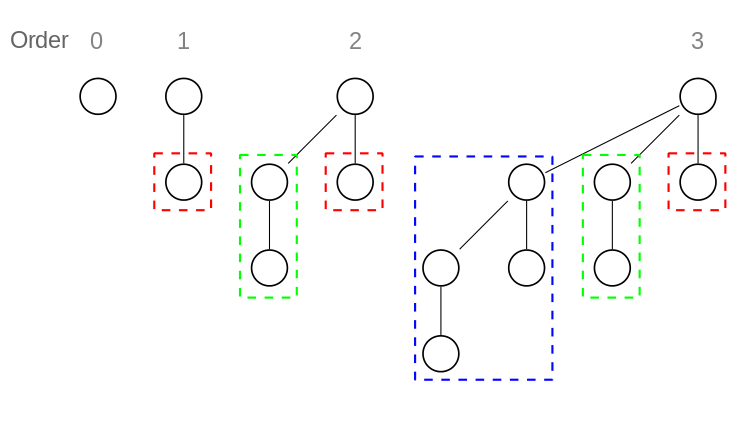
\includegraphics[width=0.5\textwidth]{binomialtree_orders}
			\caption{Verschillende ordes van binomiaalbomen.}
			\label{fig:binomialtree_orders}
		\end{figure}

\subsection{Operaties}
		\begin{itemize}
			\item \textbf{Minimum vinden}: Overloop de wortel van elke binomiaalboom. Het minimum kan ook gewoon bijgehouden worden.
			\item \textbf{Samenvoegen}: Tel de bomen met dezelfde hoogte bij elkaar op, $B_h + B_h = B_{h + 1}$. Maak de wortel met de grootste sleutel het kind van deze met de kleinste. Bij het optellen moet er wel rekening gehouden worden met eventuele overdrachten.
			\begin{itemize}
				\item \textbf{Voorbeeld}:
				\item Er is een prioriteitswachtrij met 23 elementen = $\langle B_4, B_2, B_1, B_0\rangle$
				\item Er is een prioriteitswachtrij met 13 elementen = $\langle B_3, B_2, B_0\rangle$
				\item Optellen geeft:
				\begin{table}[ht]
					\centering
					\begin{tabular}{c c c c c c}
							   & {\tiny$B_4$} & {\tiny$B_3$}      & {\tiny$B_2$} & {\tiny$B_1$} &    \\
							   \hdashline
						      & $B_4$ &       & $B_2$ & $B_1$ & $B_0$  \\
							  &       & $B_3$ & $B_2$ &       & $B_0$ \\
							  \hline
						$B_5$ &		  &		  & $B_2$ &       &		 			
					\end{tabular}
					\caption{De binomiaalbomen boven de gestreepte lijn duiden de overdrachten aan.}
				\end{table}
			\end{itemize}
			
			
			Figuur \ref{fig:binomialtree_fig} toont de samenvoegoperatie voor twee $B_2$ bomen.
			\begin{figure}[ht]
				\centering
				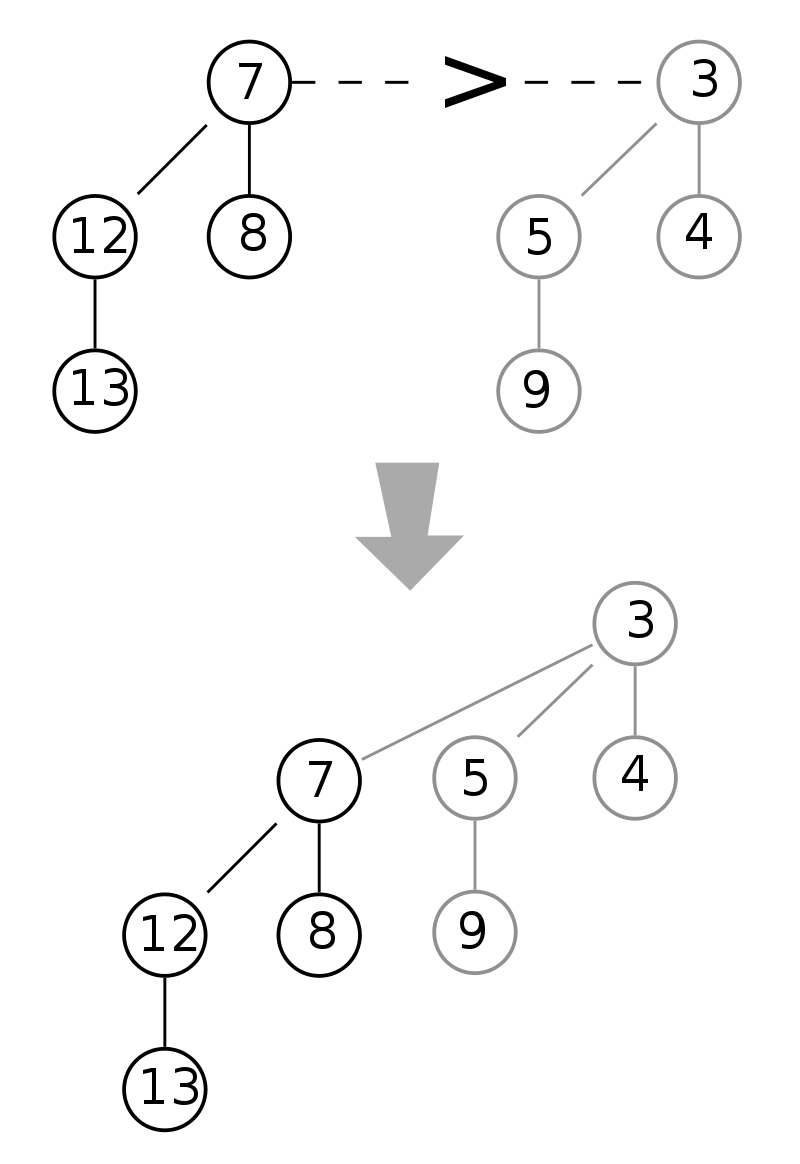
\includegraphics[width=0.3\textwidth]{binomialtree_merge}
				\caption{Hier worden twee binomiaalbomen $B_2$ samengevoegd. De boom met de waarde 7 voor de wortel wordt het linkerkind van de boom met waarde 3 voor de wortel. Het wordt een boom van orde $B_3$.}
				\label{fig:binomialtree_fig}
			\end{figure}
			\item \textbf{Toevoegen}: Maak een triviale binomiaalqueue met één knoop en voeg deze samen met de andere binomiaalqueue.
			\item \textbf{Minimum verwijderen}: Zoek binomiaalboom $B_k$ met het kleinste wortelelement. Verwijder deze uit de binomiaalqueue. De deelbomen van deze binomiaalboom vormen een nieuw binomiaalbos die samengevoegd kan worden met de originele heap.
		\end{itemize}

\section{Pairing heaps}
		\begin{itemize}
			\item Een algemene boom waarvan de sleutels voldoen aan de heapvoorwaarde.
			\item Elke knoop heeft een wijzer naar zijn linkerkind en rechterbroer (figuur \ref{fig:pairingheap} en \ref{fig:pairingheap_treeform}). Als verminderen van prioriteit moet ondersteund worden, heeft elke knoop als linkerkind een wijzer naar zijn ouder en als rechterkind een wijzer naar zijn linkerkind.
		\end{itemize}
		\begin{figure}[ht]
			\centering
			\begin{minipage}{.49\textwidth}
				\centering
				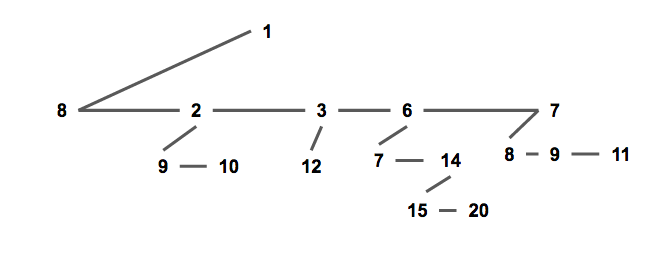
\includegraphics[width=\linewidth]{pairingheap}
				\caption{Een pairing heap.}
				\label{fig:pairingheap}
			\end{minipage}
			\begin{minipage}{.49\textwidth}
				\centering
				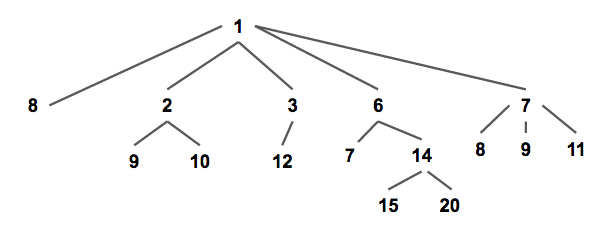
\includegraphics[width=\linewidth]{pairingheap_treeform}
				\caption{Dezelfde pairing heap, maar in boomvorm.}
				\label{fig:pairingheap_treeform}
			\end{minipage}%
		\end{figure}

		De \underline{operaties} op een pairing heap.
		\begin{itemize}
			\item \textbf{Samenvoegen}: Verlijk het wortelelement van beide heaps. De wortel met het grootste element wordt het linkerkind van deze met het kleinste element.
			\item \textbf{Toevoegen}: Maak een nieuwe pairingheap met één element, en voeg deze samen met de oorspronkelijke heap.
			\item \textbf{Prioriteit verminderen}: De te wijzigen knoop wordt losgekoppeld, krijgt de prioriteitwijziging, en wordt dan weer samengevoegd met de oorspronkelijke heap.
			\item \textbf{Minimum verwijderen}: De wortel verwijderen levert een collectie van $c$ heaps op. Voeg deze heaps van links naar rechts samen in $O(n)$ of voeg eerst in paren toe, en dan van rechts naar links toevoegen in geamortiseerd $O(\lg n)$.
			\item \textbf{Willekeurige knoop verwijderen}: De te verwijderen knoop wordt losgekoppeld, zodat er twee deelheaps onstaan. Deze twee deelheaps worden samengevoegd.
		\end{itemize}
